\iffalse
\documentclass[epj,nopacs,fleqn]{svjour}
\smartqed
\usepackage[T1]{fontenc}
\usepackage[utf8]{inputenc}
\usepackage{cite,epsfig,amsmath,graphicx,amssymb,listings,slashed}
\usepackage[colorlinks,citecolor=blue,urlcolor=blue,linkcolor=blue]{hyperref}
\journalname{Eur. Phys. J. C}

\title{MadDM 3.0 EW}
\author{
  Federico Ambrogi\inst{1},
}
\institute{
University of Vienna, Faculty of Physics, Bolzmanngasse 5, A-1090 Wien, Austria \\
email: {\color{blue}federico.ambrogi88@gmail.com}
}

\date{Received: date / Accepted: date}
\titlerunning{MadDM 3.0 EW}
\authorrunning{F.~Ambrogi \textit{et al.}}



\fi

\documentclass[a4paper,11pt]{article}
%\pdfoutput=1 % if your are submitting a pdflatex (i.e. if you have
             % images in pdf, png or jpg format)
\usepackage{jheppub} % for details on the use of the package, please
                     % see the JHEP-author-manual
\usepackage[T1]{fontenc} % if needed
\usepackage{booktabs}

\usepackage{slashed}
%\usepackage{subfigure}
\usepackage{xspace}
\usepackage{booktabs}
%% %simple case: 2 authors, same institution
%% \author{A. Uthor}
%% \author{and A. Nother Author}
%% \affiliation{Institution,\\Address, Country}

\begin{document}
\title{\boldmath MadDM 3.0 EW}

\author[a]{Federico Ambrogi}
\affiliation[a]{University of Vienna, Faculty of Physics, Bolzmanngasse 5, A-1090 Wien, Austria}
% e-mail addresses: one for each author, in the same order as the authors\emailAdd{federico.ambrogi@oeaw.ac.at}
\emailAdd{federico.ambrogi88@gmail.com}

\maketitle




\newcommand{\PPPC}{\texttt{PPPC4DMID}}
\newcommand{\PPPCew}{\texttt{PPPC4DMID\_ew}}
\newcommand{\MG}{\texttt{MadGraph5\_aMC@NLO}}


\newcommand{\run}{\texttt{run\_card.dat}}
\newcommand{\param}{\texttt{param\_card.dat}}
\newcommand{\mchi}{$m_{\chi _D}$}


\section*{Abstract}
This documents summarises the status of the studies of the discrepancies found in the energy spectra provided in the PPPC4DMID tables (labelled \textbf{PPPC4DMIDew} in MadDM v.3.0) and the spectra produced with MadDM 3.0.



\section{Introduction}
All the information, including the model used and the input cards (\run~ ,\param) can be found at:
\\
{\color{blue} \url{ https://github.com/fambrogi/MadDM} }

\clearpage
\section{PPPC Electroweak Corrections}
In this section the energy spectra for the Cosmic Rays $CRs = e^+, \nu_e , \gamma$ extracted from the \PPPC~and \PPPCew~ Tables are compared, to get an idea of the effect of the EW correction (according the \PPPC collaboration). 

\begin{figure}[!]
\begin{center}
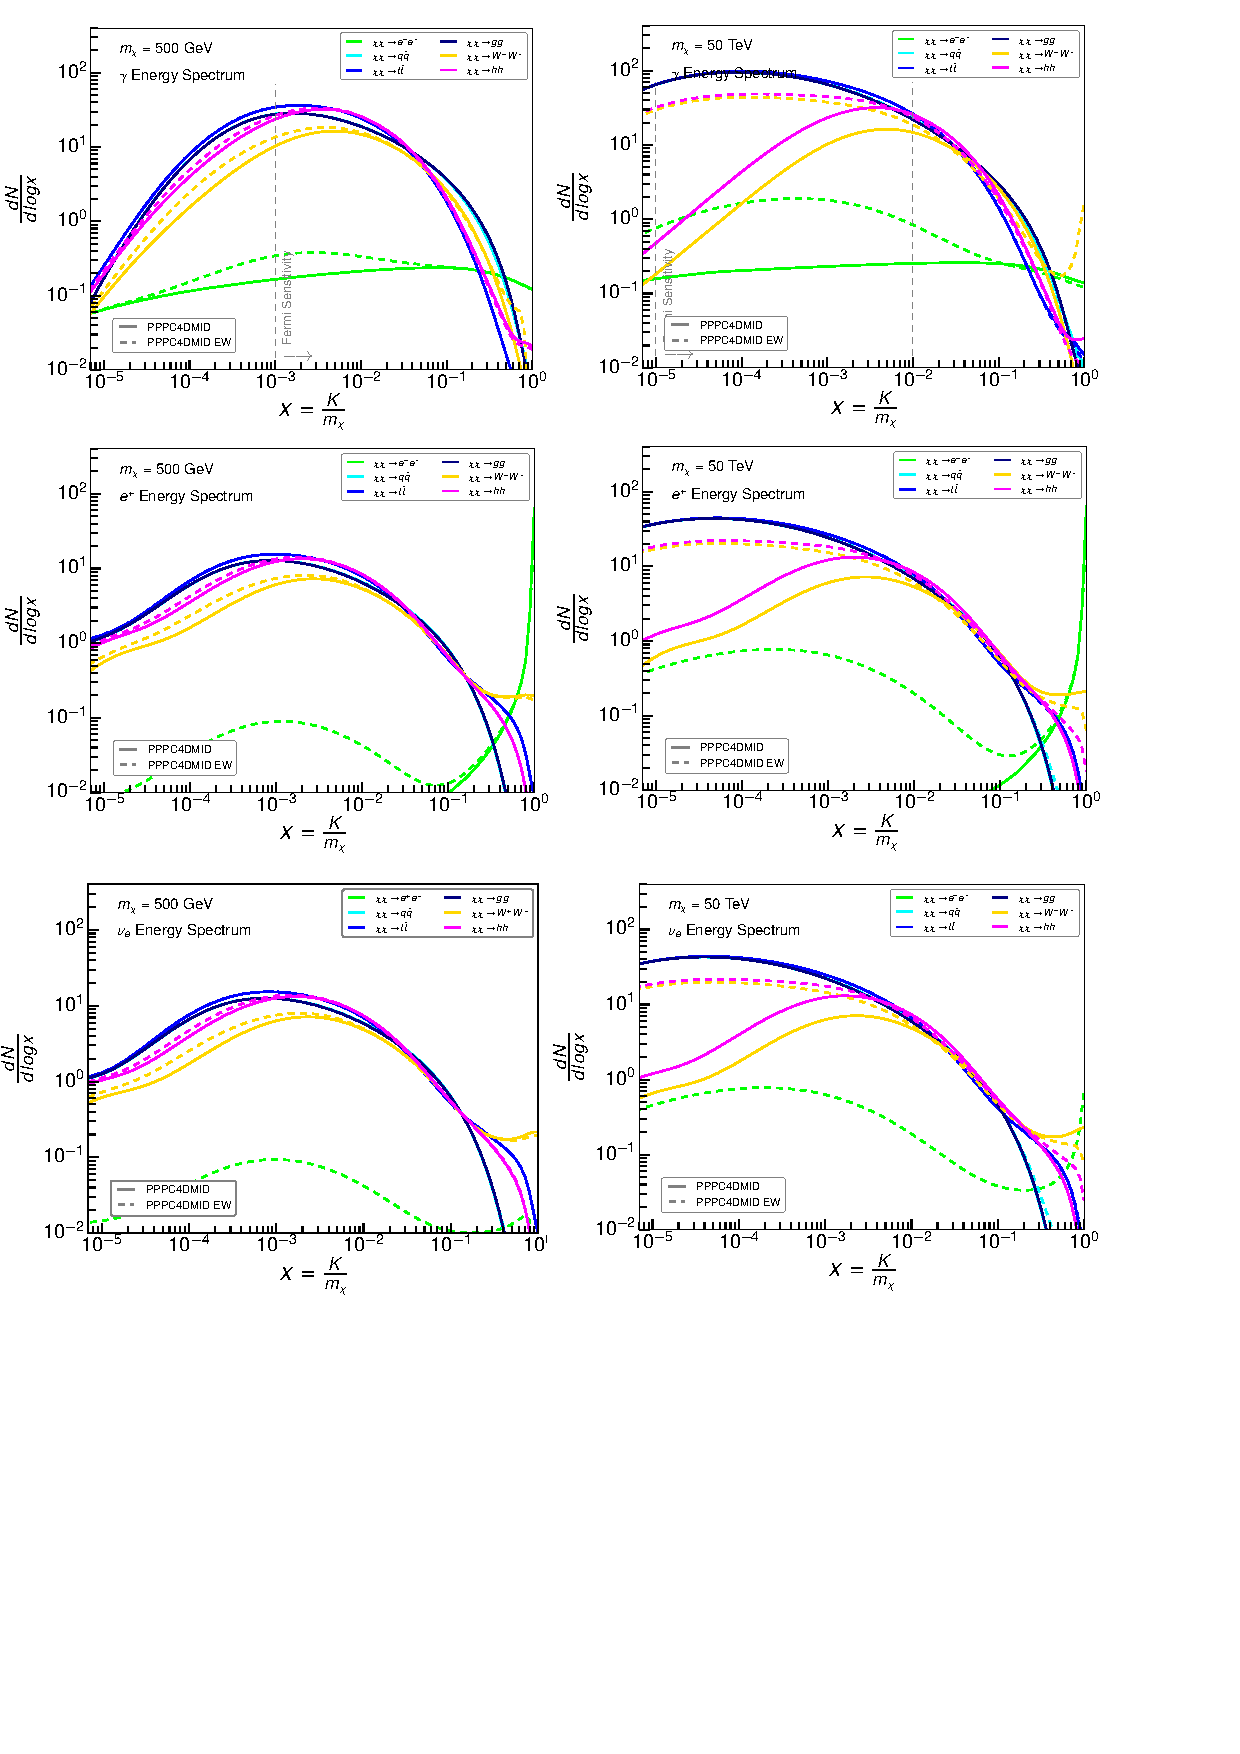
\includegraphics[width=1\textwidth]{Fig/EW_noEW_PPPC.pdf}
\end{center}
\caption{Energy spectra ($\gamma, e^+, \nu _e$) for $m_{\chi}=$500 GeV (left) and 50 TeV (right) extracted from the \PPPC~and \PPPCew~tables, for selected annihilation channels.}
\end{figure}


\clearpage
\section{EW with \MG}
\subsection{Processes}
The processes used for the production of the samples with emission of extra electroweak bosons (Higgs, W and Z bosons) are the following:
\begin{verbatim}
import model DMsimp_s_spin0_EW
define X = W- W+ Z h
generate xd xd~ > w- w+
add process xd xd~ > w- w+ X
add process xd xd~ > w- w+ X X
add process xd xd~ > w- w+ X X X
\end{verbatim}
Note that the short notation e.g. "XXW" includes the lower order processes (in this case only the tree level xdxd>WW) and up to one extra "X" boson, and likewise for the higher order processes. \\

Syntax for excluding diagrams with photons:
\begin{verbatim}
import model DMsimp_s_spin0_EW
define X = W- W+ Z h
generate xd xd~ > w- w+ /a
add process xd xd~ > w- w+ X  /a
add process xd xd~ > w- w+ X X  /a
add process xd xd~ > w- w+ X X X  /a
\end{verbatim}
\\

Relevant parameters in the \run~: 
\begin{verbatim}
*** run_card
1001.0     = ebeam1  
10001.0    = ebeam1  
100001.0    = ebeam1 
\end{verbatim}
for  $m_{\chi_D}$=1 , 10, 100 TeV respectively, and the \param~:
\begin{verbatim}
*** param_card
52 1.00000e+03 # MXd 
54 2.00000e+03 # MY0  (= 2 x MXd )   
\end{verbatim}
\\

\subsection{Cross Sections Comparison}
In Tab. \ref{xsec} the cross sections in [pb] obtained with different runs are shown.
\begin{table*}[!h]
\centering
\renewcommand{\arraystretch}{1.2}
\small
\begin{tabular}{ l | c | c | c | c } \toprule \toprule 
$\mathbf{m_{\chi_D}} $ & $\mathbf{\chi _D \chi _D \rightarrow WW} $ & $\mathbf{\chi _D \chi _D \rightarrow WW X} $ & $\mathbf{\chi _D \chi _D \rightarrow WWX X }$ & $\mathbf{\chi _D \chi _D \rightarrow WW X X X}$ \\  \toprule 
    1.0 TeV (Old) & 474 & 130* & 600 & 600 \\  
    1.0 TeV (Old, no $\gamma$) & 474 & 676 & 704 & - \\  
    1.0 TeV (New) & 173 & 215 & 219 & - \\  
    1.0 TeV (New,AUTO) & 147.3 & 148.2 & - & - \\    

    1.0 TeV (Chiara) & 147.3 & 148.2 & 148.2 & - \\    

  
  10.0 TeV (Old)  & 15.1 $\times 10 ^3$ & 30.501 $\times 10 ^3$ & 37.018 $\times 10 ^3$ & - \\ 
  10.0 TeV (Old,no $\gamma$)  & 15.1 $\times 10^3$  & 2.7 $\times 10 ^7$ & 1.5 $\times 10^{10}$ & - \\ 

  10.0 TeV (New)  & 15.1 $\times 10 ^3$ & 30.542 $\times 10 ^3$  & - & - \\    
  100.0 TeV (Old) & 4.7  $\times 10 ^5$  & - & - & - \\  



    \bottomrule \bottomrule
  \end{tabular}
  \caption{Cross sections in [pb]  for various processes extracted from the LHE files. The "New" cross sections were computed with $N_{Events}$=10,000, while the "Old" ones with $N_{Events}$=100,000. Need to verify the value 130*. }
  \label{xsec}
\end{table*}



\clearpage
\subsection{Spectra for $\chi_D \chi_D \rightarrow WW$}
\subsubsection{$m_{\chi_D}$ = 1 TeV}
\begin{figure}[!b]
\centering
\subfigure
{ 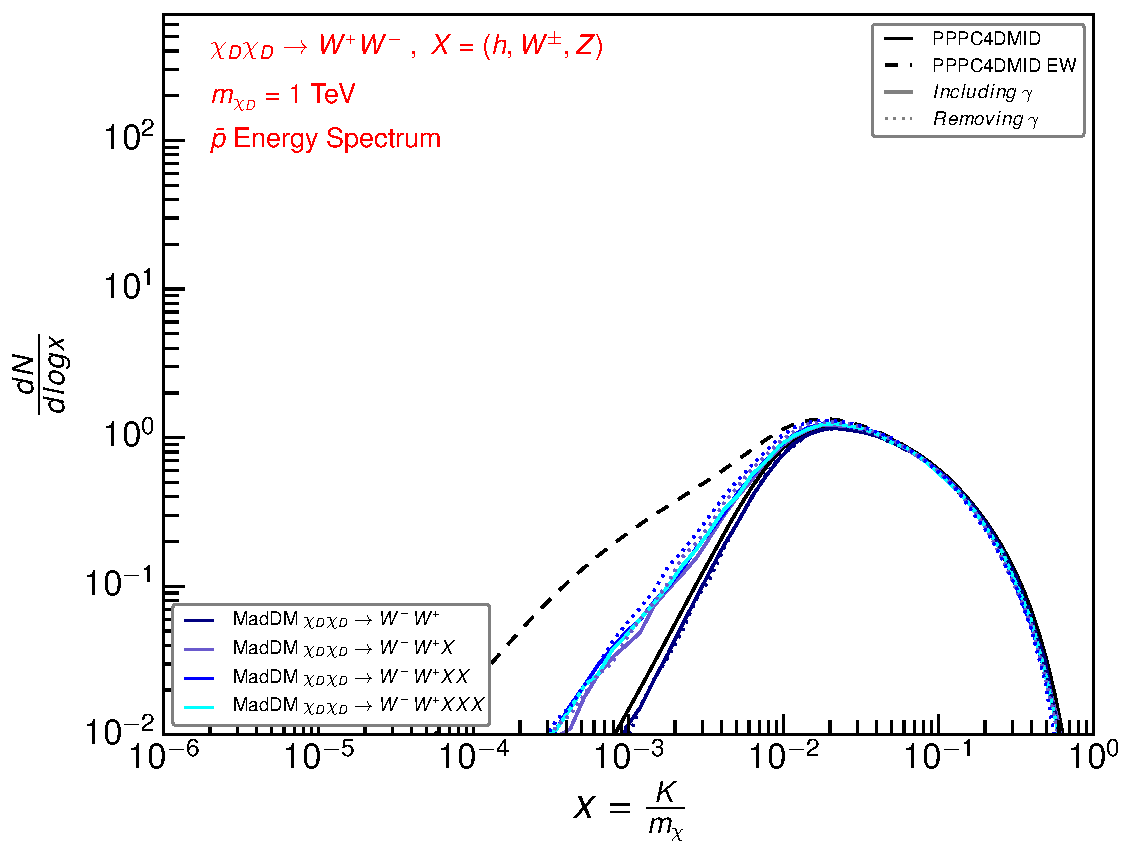
\includegraphics[width=0.49\textwidth]{Fig/1TeV/1_antiprotons_PPPC_Comparison_xdxd_fotone_1.pdf}}
\subfigure
{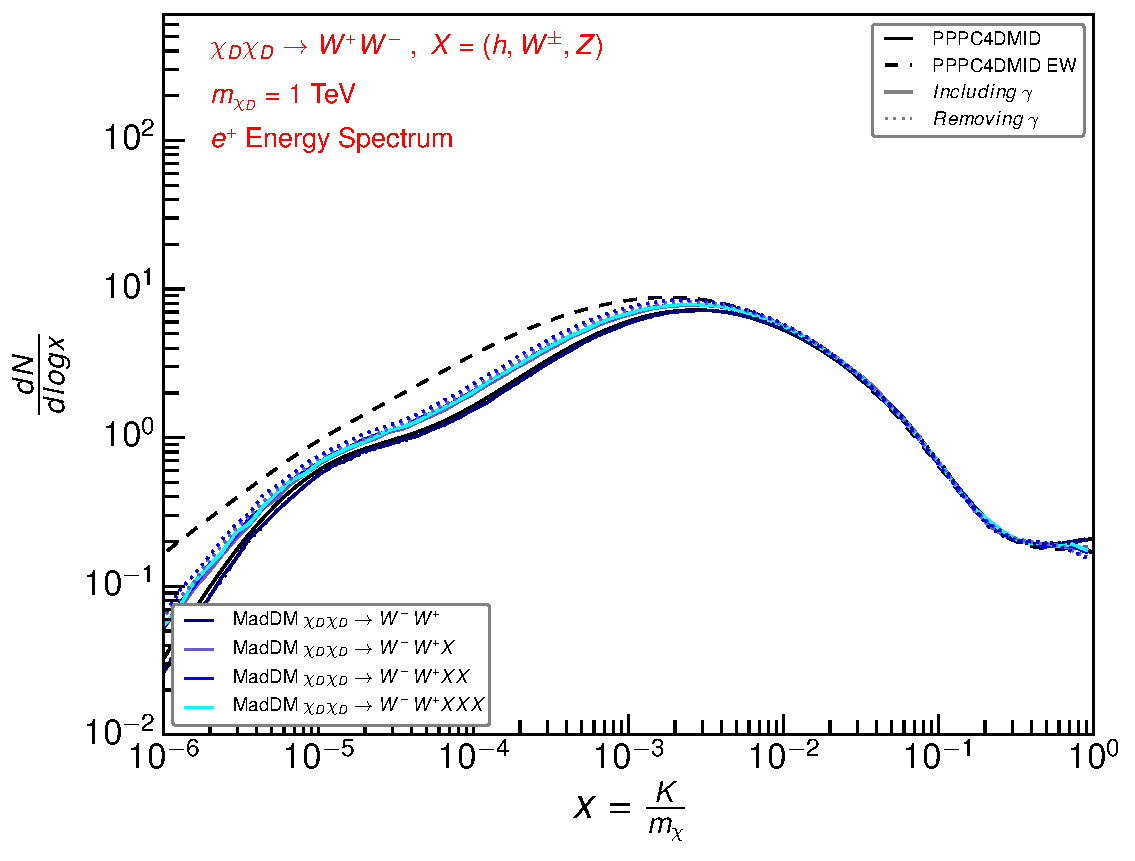
\includegraphics[width=0.49\textwidth]{Fig/1TeV/1_positrons_PPPC_Comparison_xdxd_fotone_1.pdf}}
\subfigure
{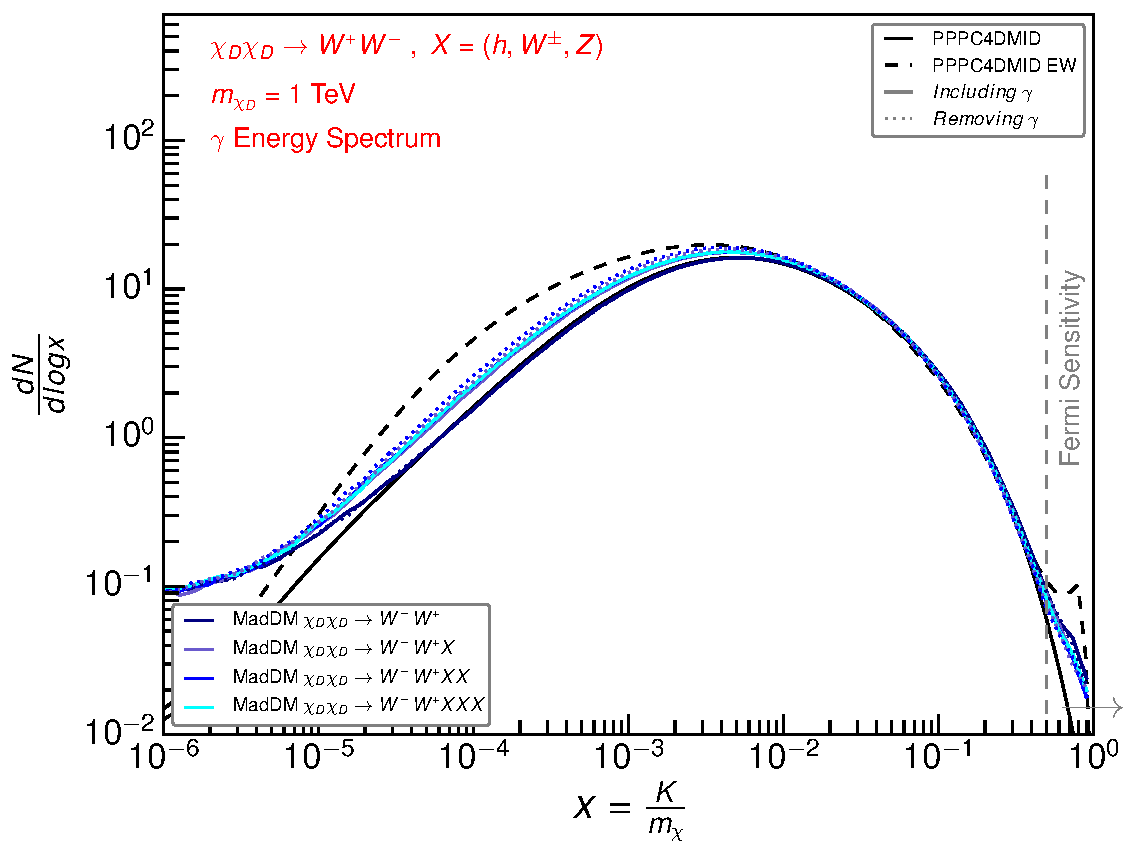
\includegraphics[width=0.49\textwidth]{Fig/1TeV/1_gammas_PPPC_Comparison_xdxd_fotone_1.pdf}}
\subfigure
{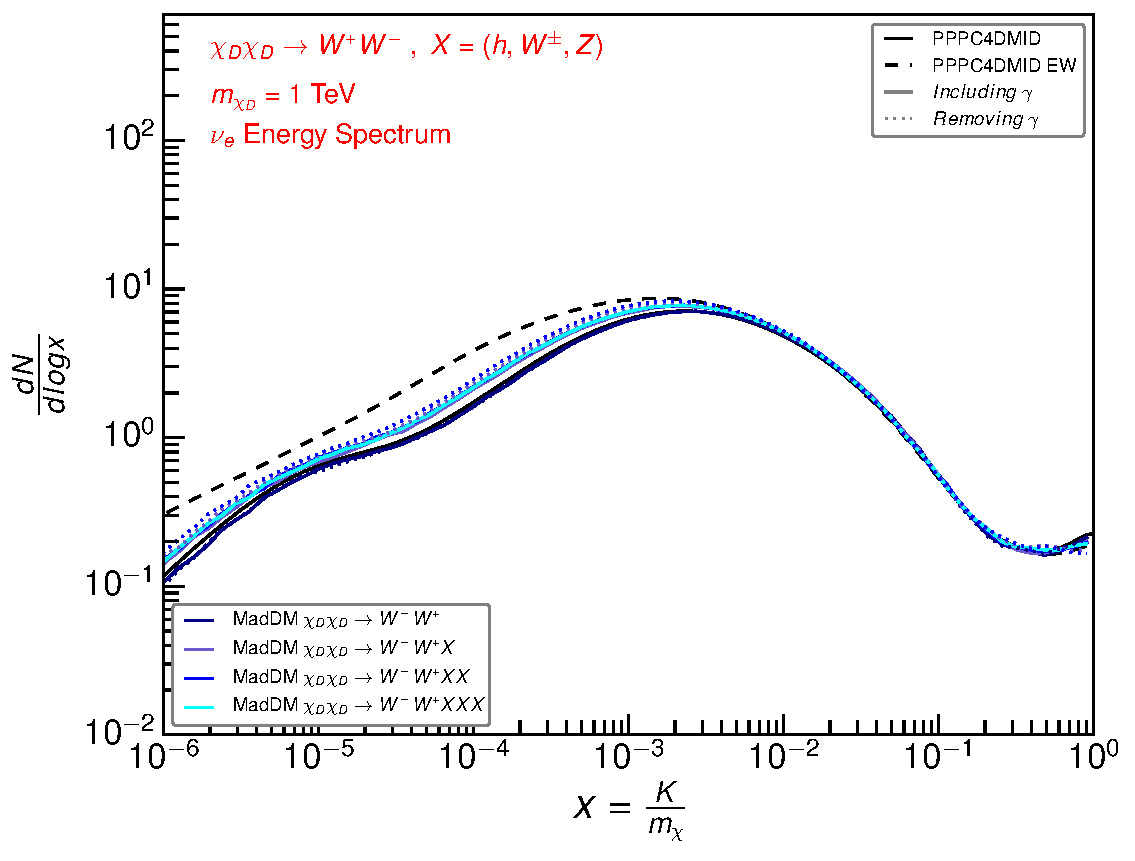
\includegraphics[width=0.49\textwidth]{Fig/1TeV/1_neutrinos_e_PPPC_Comparison_xdxd_fotone_1.pdf}}
\subfigure
{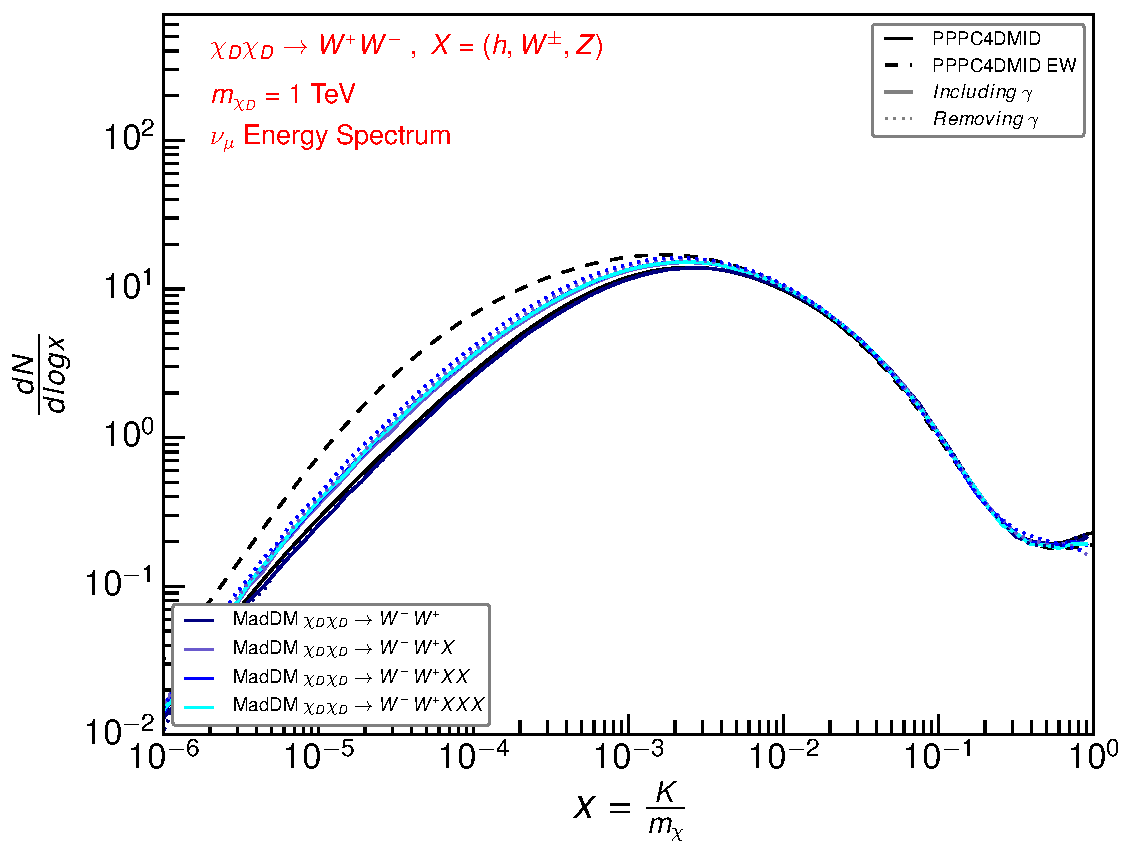
\includegraphics[width=0.49\textwidth]{Fig/1TeV/1_neutrinos_mu_PPPC_Comparison_xdxd_fotone_1.pdf}}
\subfigure
{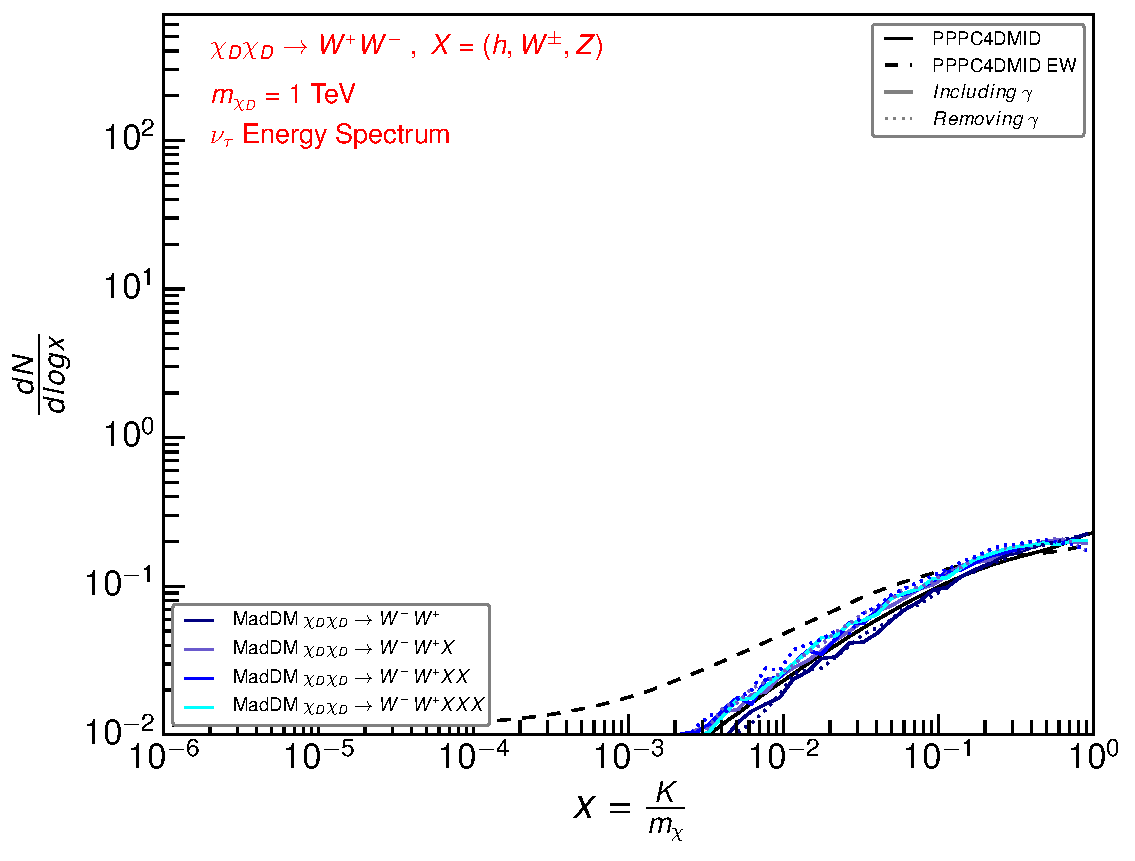
\includegraphics[width=0.49\textwidth]{Fig/1TeV/1_neutrinos_tau_PPPC_Comparison_xdxd_fotone_1.pdf}}
\caption{Energy Spectra for $m_{\chi_D}$ = 1 TeV}
\end{figure}
%
%
%
\clearpage
\subsubsection{"Old" $m_{\chi_D}$ = 100 TeV}
\begin{figure}[!b]
\centering
\subfigure
{ 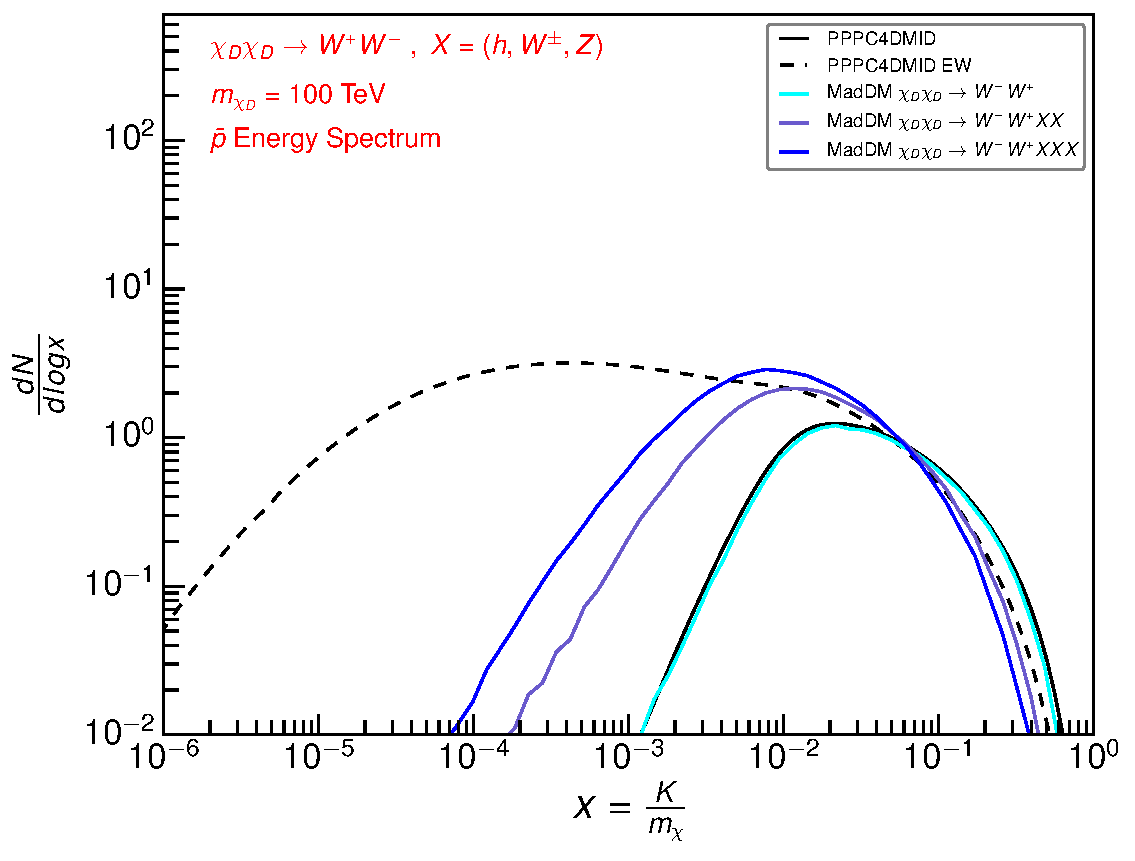
\includegraphics[width=0.49\textwidth]{Fig/100TeV_OLD/OLD_100000_antiprotons_PPPC_Comparison_xdxd_100000.pdf}}
\subfigure
{ 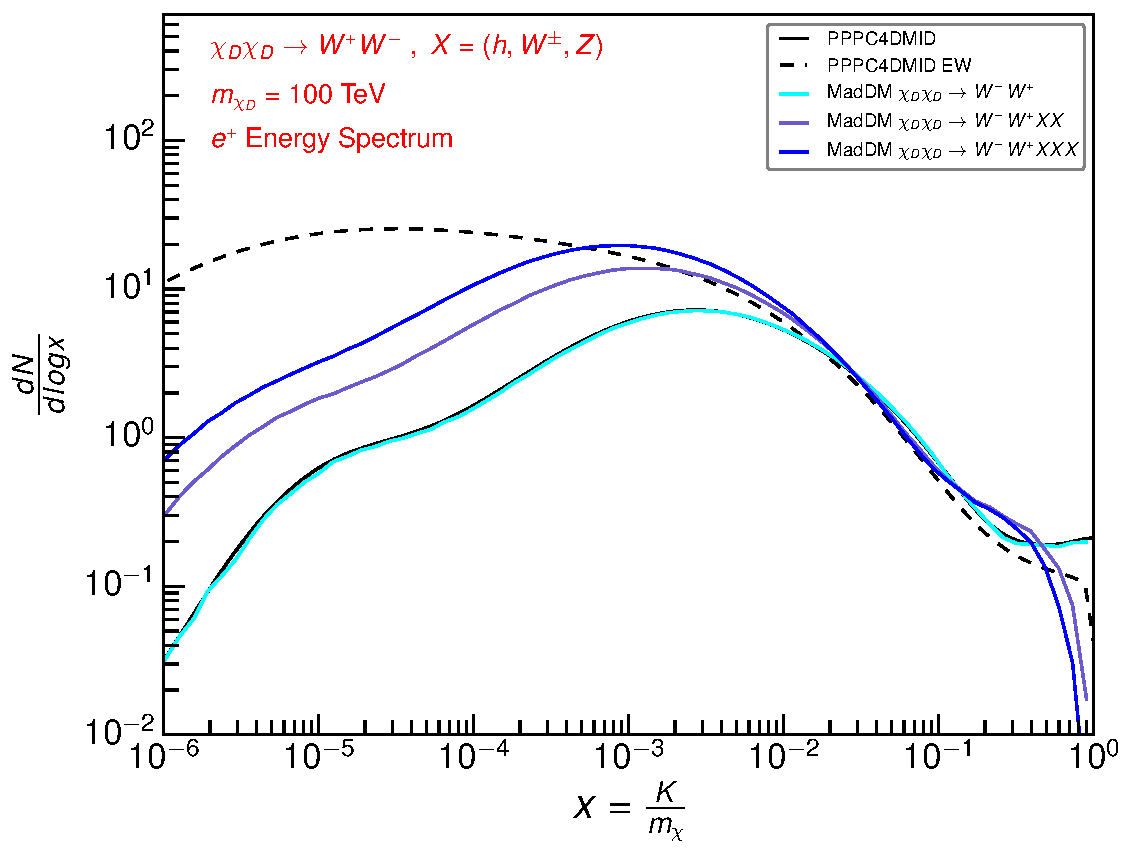
\includegraphics[width=0.49\textwidth]{Fig/100TeV_OLD/OLD_100000_positrons_PPPC_Comparison_xdxd_100000.pdf}}
\subfigure
{ 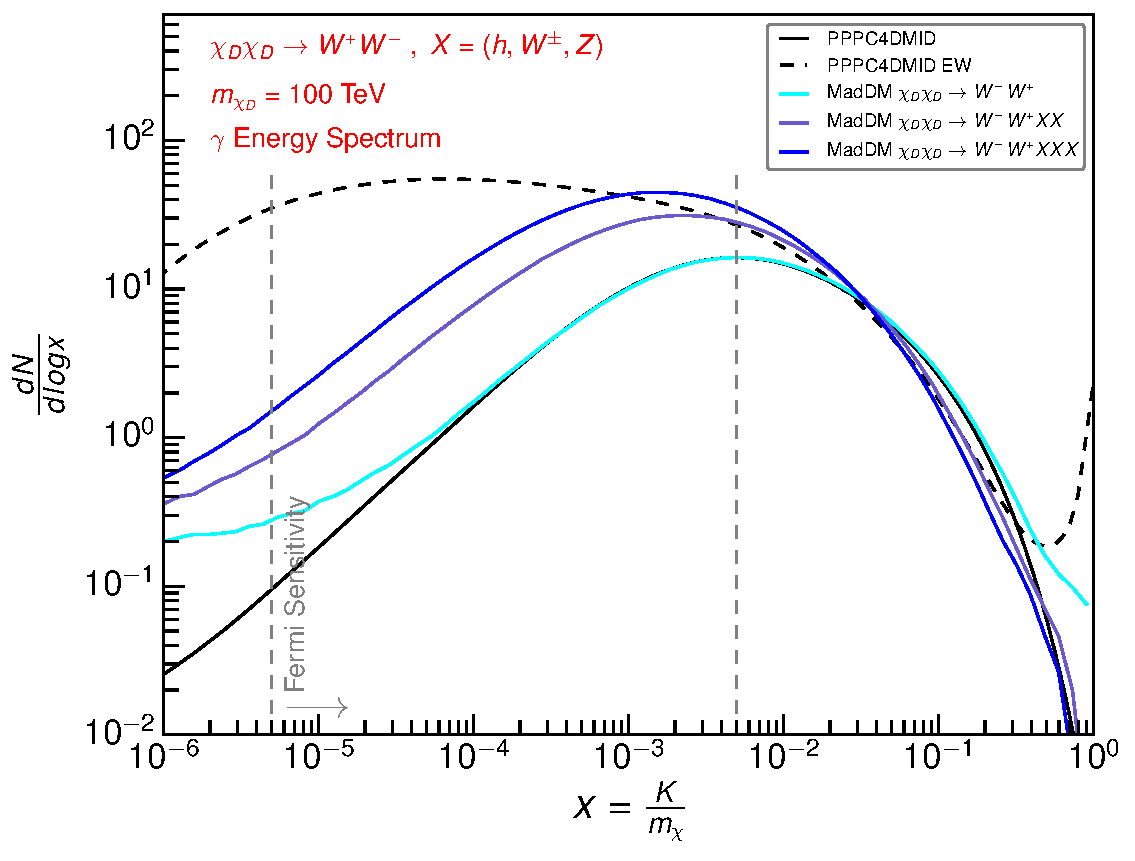
\includegraphics[width=0.49\textwidth]{Fig/100TeV_OLD/OLD_100000_gammas_PPPC_Comparison_xdxd_100000.pdf}}
\subfigure
{ 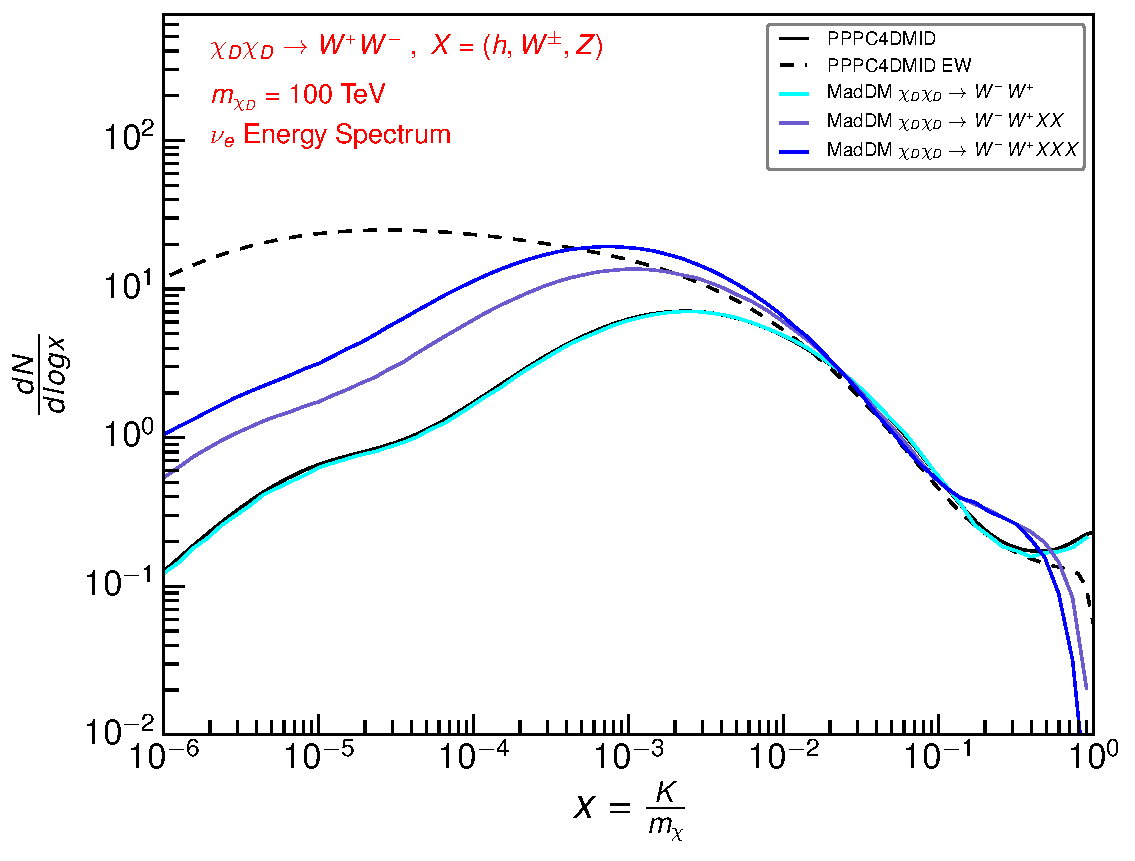
\includegraphics[width=0.49\textwidth]{Fig/100TeV_OLD/OLD_100000_neutrinos_e_PPPC_Comparison_xdxd_100000.pdf}}
\subfigure
{ 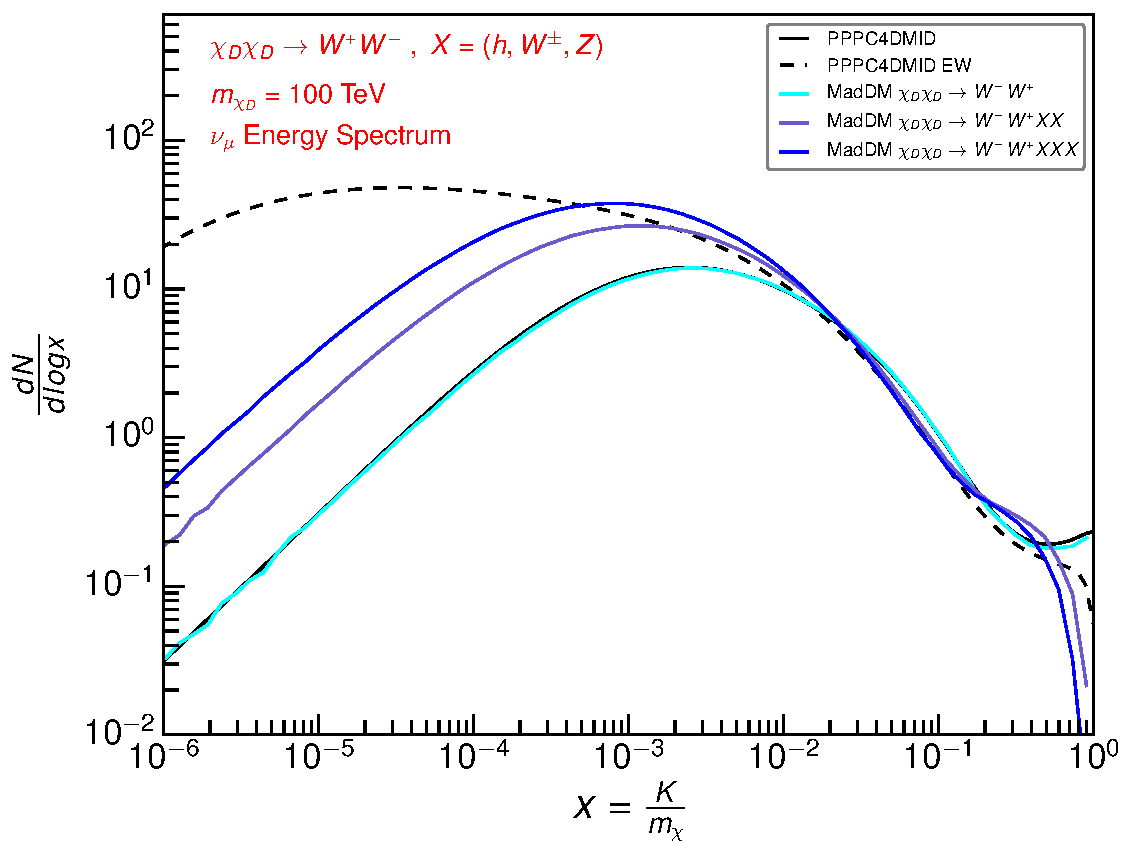
\includegraphics[width=0.49\textwidth]{Fig/100TeV_OLD/OLD_100000_neutrinos_mu_PPPC_Comparison_xdxd_100000.pdf}}
\subfigure
{ 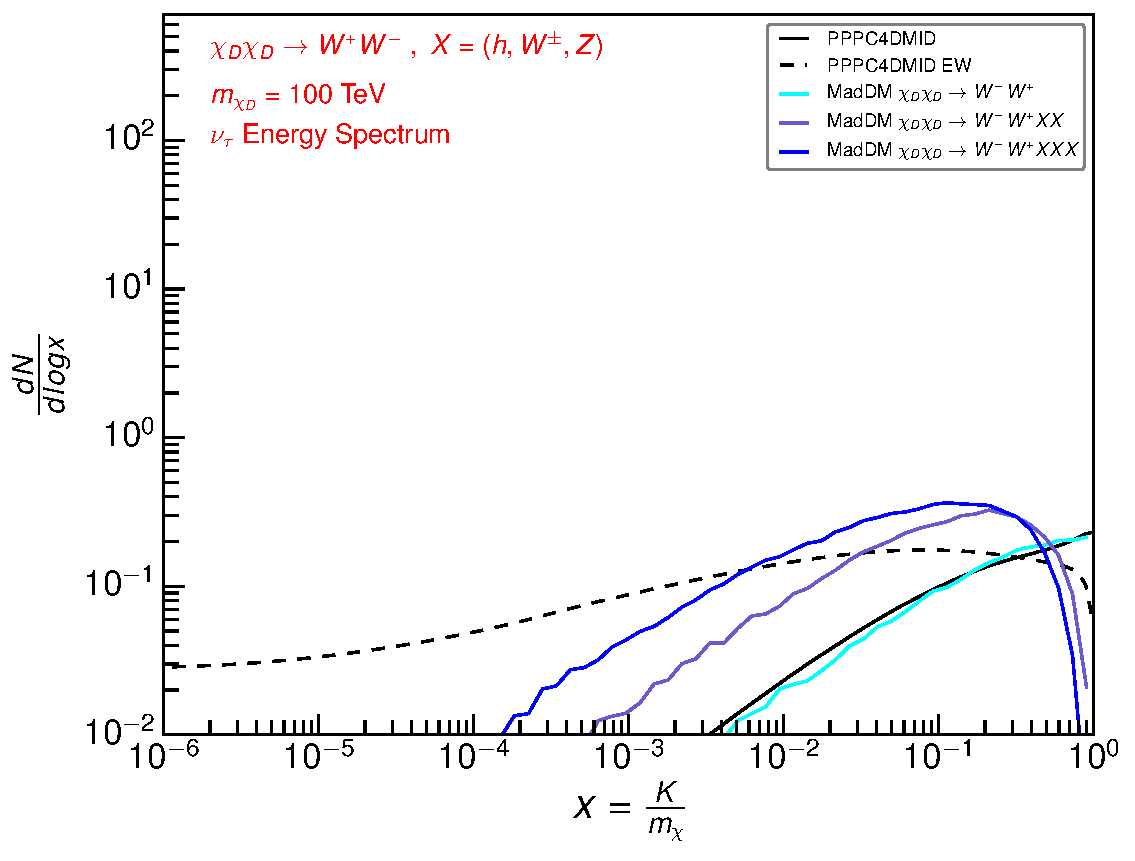
\includegraphics[width=0.49\textwidth]{Fig/100TeV_OLD/OLD_100000_neutrinos_tau_PPPC_Comparison_xdxd_100000.pdf}}
\caption{Energy Spectra for $m_{\chi_D}$ = 100 TeV (Old data)}
\end{figure}
%

\clearpage
\subsection{Spectra for $\chi_D \chi_D \rightarrow Y0 \rightarrow FFFF$}

Here the spectra for the process $\chi_D \chi_D \rightarrow Y0 \rightarrow FFFF$ are shown for $m_{\chi_D}$ = 1 TeV, compared to the \PPPC and \PPPCew~ spectra. To produce the sample, the EW model was modified adding masses to the light quarks and muons, otherwise there is a problem in \MG~when evaluating the cross sections (re-using the same diagrams with masless particles?). I used the value of the muon mass (0.105 GeV) for the light quarks, and 4.5 GeV for the bottoms. \\

The model can be found at {\color{blue} \url{https://github.com/fambrogi/MadDM/tree/master/EW_Study/EW_Model_FermionMass}}, while the complete banner can be found in {\color{blue} \url{https://github.com/fambrogi/MadDM/blob/master/EW_Study/Banners/xdxd_Y0_FFFF_1TeV_banner.dat} }.
\\


\MG~ Process:
\begin{verbatim}
import model DMsimp_s_spin0_EW_MM
define F = ve vm vt e- mu- ve~ vm~ vt~ e+ mu+ t t~ u c d s b u~ c~ d~ \
s~ b~ ta- ta+
generate xd xd~ > y0 > F F F F
output xdxd_Y0_FFFF
\end{verbatim}
%
\\


Pythia8 cards commands:
\begin{verbatim}
TimeShower:weakShower = on (or off)
WeakShower:singleEmission = off
\end{verbatim}



\begin{figure}[!b]
\centering
\subfigure
{ 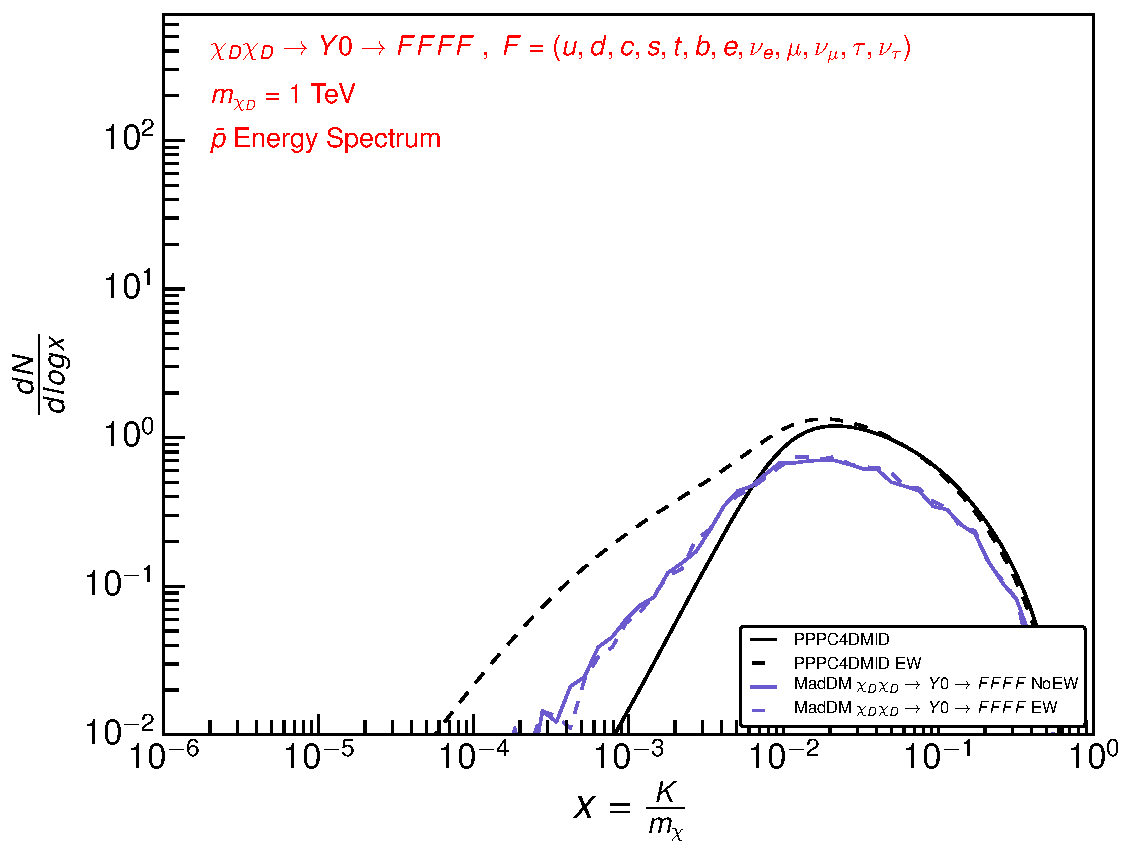
\includegraphics[width=0.49\textwidth]{Fig/xdxd_Y0/1_antiprotons_FFFF_xdxd_1.pdf}}
\subfigure
{ 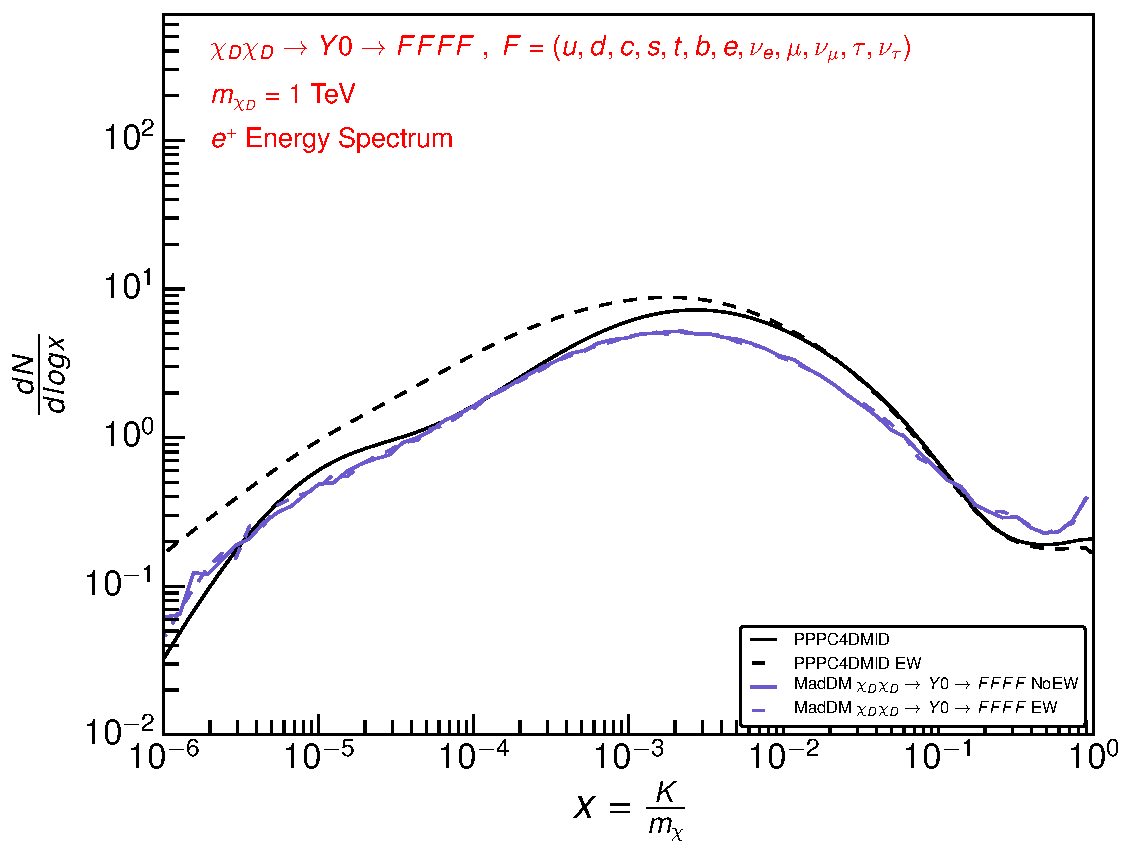
\includegraphics[width=0.49\textwidth]{Fig/xdxd_Y0/1_positrons_FFFF_xdxd_1.pdf}}
\subfigure
{ 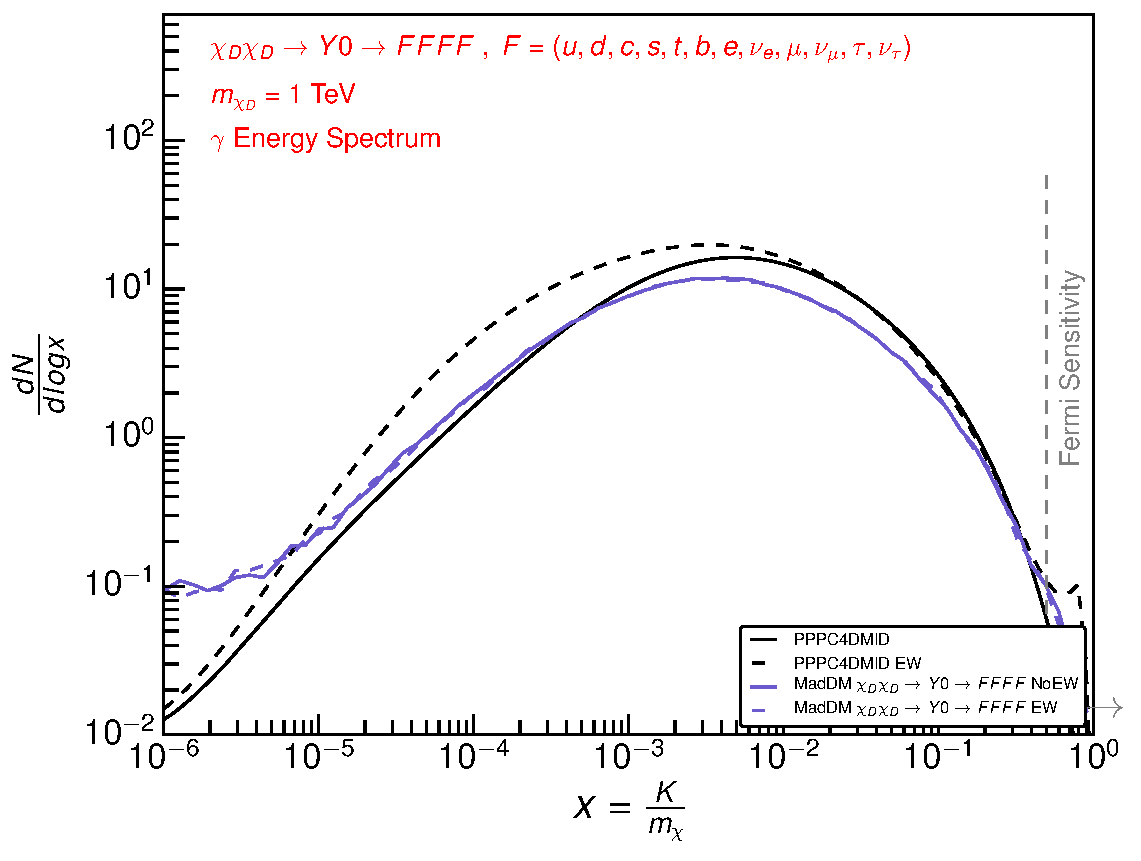
\includegraphics[width=0.49\textwidth]{Fig/xdxd_Y0/1_gammas_FFFF_xdxd_1.pdf}}
\subfigure
{ 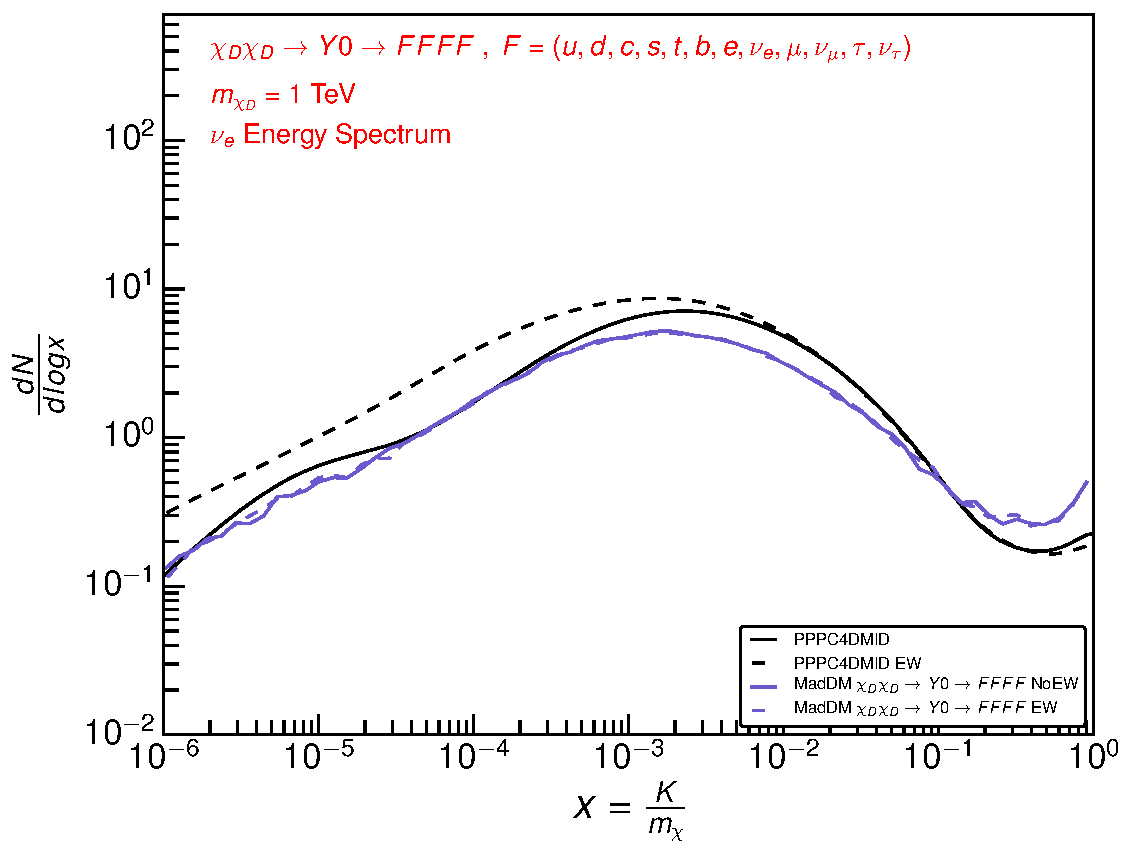
\includegraphics[width=0.49\textwidth]{Fig/xdxd_Y0/1_neutrinos_e_FFFF_xdxd_1.pdf}}
\subfigure
{ 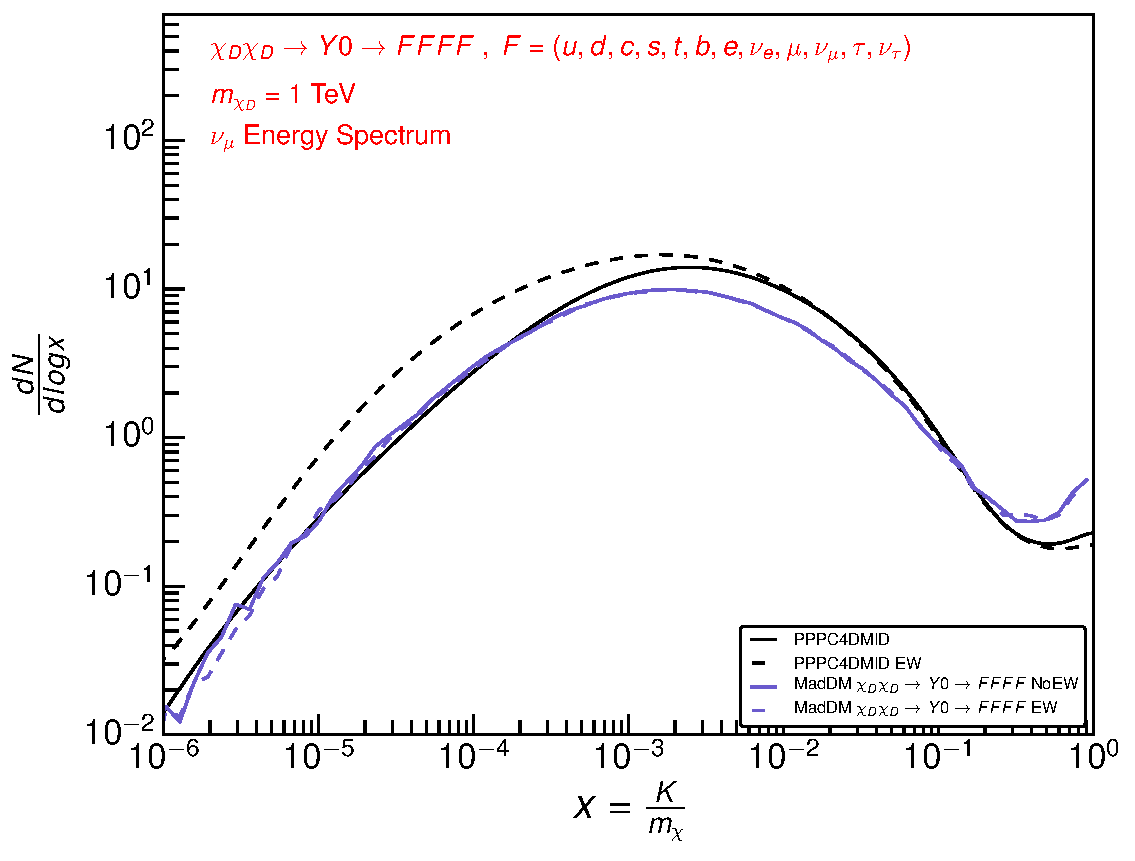
\includegraphics[width=0.49\textwidth]{Fig/xdxd_Y0/1_neutrinos_mu_FFFF_xdxd_1.pdf}}
\subfigure
{ 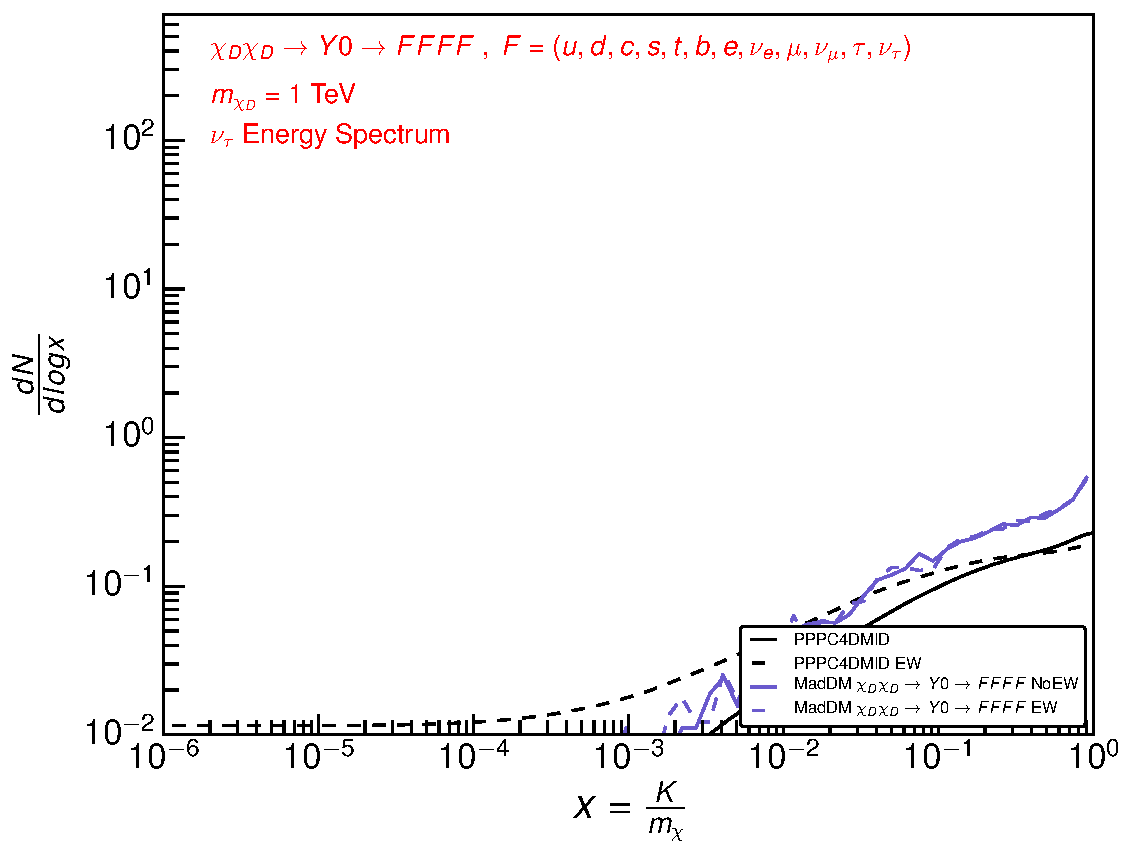
\includegraphics[width=0.49\textwidth]{Fig/xdxd_Y0/1_neutrinos_tau_FFFF_xdxd_1.pdf}}
\caption{Energy Spectra for $m_{\chi_D}$ = 1 TeV (Old data) for the process $\chi_D \chi_D \rightarrow Y0 \rightarrow FFFF$. The label "EW" and "NoEW" in the MadDM samples mean respectively samples produced with or without the EW corrections in Pythia8.}
\end{figure}

\clearpage
\section{MG5 Issues}
Sometimes, but not always, I get the following message:
\begin{verbatim}
INFO: Combining Events 
INFO: fail to reach target 10000 
  === Results Summary for run: run_01 tag: tag_1 ===

     Cross-section :   2.711e+06 +- 6.486e+04 pb
     Nb of events :  25
\end{verbatim}
when generating events with extra bosons for \mchi = 100 TeV. The \MG~ version is 2.6.4 .
\clearpage



\section*{Acknowledgments}
Thanks
%
\bibliographystyle{JHEP}
\bibliography{references}

\end{document}
